
Man kan nu begynde at anvende de ligninger der er blevet udledt i de tidligere afsnit, på en cylinder.
\\
Der er givet en cylinders parameterfrenstilling:

\begin{equation}
r(\theta)=(cos(\theta),sin(\theta),z)
\end{equation}
\\
En geodætisk kurve henover denne cylinder kunne se således ud:
\\
\begin{equation}
r(\theta):=(cos(\theta),sin(\theta),z(\theta))
\end{equation}
\\
Afstanden hen over cylinderen er givet ved Lagrangefunktionen, hvor S er et udtryk for længden
\begin{equation}
S = \sqrt{(\frac{d}{d\theta}cos(\theta))^2+\frac{d}{d\theta}sin(\theta))^2+\frac{d}{d\theta}z(\theta))^2}d\theta
\end{equation}
\\
Simplificerer vi dette en smule får vi:
\begin{equation*}
S=\int_{\theta_a}^{\theta_b}\sqrt{(1+\dot{z}(z(\theta))^2}
\end{equation*}
\\
Hertil kan vi definerer funktionen der beskriver den differenterede længde.
\begin{equation*}
S=\sqrt{(1+(z(\theta))^2}
\end{equation*}
Skal S være så lille som muligt skal f dertil opfylder Euler-Lagrange differentialligning
\begin{equation}
\frac{\partial f}{\partial z}-\frac{d f}{d \theta} \frac{d f}{d\dot{z}}=0
\end{equation}
Da $\frac{\partial f}{\partial z}$ bliver Euler-lagrange ligning da:
\begin{equation}
\int_{\theta_a}^{\theta_b}\frac{d}{d\theta}\frac{\dot{z}\theta}{\sqrt{(1+\dot{z}(z(\theta))^2}d\theta}
\end{equation}
Differeteres der i forhold til theta fås der
\begin{equation}
\int_{\theta_a}^{\theta_b}\frac{\dot{\dot{z}}\theta}{\sqrt{(1+\\dot{\dot{z}(z(\theta))^2}d\theta}}
\end{equation}
For at denne skal give 0 skal tælleren have formen:
\begin{equation}
k\cdot \theta+C = z(\theta)
\end{equation}
k er et udtryk for hældning og C er bare en konstant.
\\
Dette betyder at funktionen der forbinder 2 punkter på en cylinder er en ret linje hvilket jo også giver mening.
\\
\\
Vi kan nu opstille to ligninger til undersøgelse af hvilken effekt det vil have at ændre de forskellige parametre.
\\
Første ligning
\begin{equation}
k\cdot \theta_a + C = z(\theta_a)
\end{equation}
Anden ligning
\begin{equation}
k\cdot \theta_b + C = z(\theta_b)
\end{equation}
hvor det gælder at
\begin{equation}
\begin{gathered}
z(\theta_a)=Z_a \\
z(\theta_b)=Z_b\\
\theta_a,\theta_b,\in[0;2\pi[ \\
\theta_a < \theta_b
\end{gathered}
\end{equation}
Hældningen for en ret linje mellem 2 punkter kan udtrykkes ved $\frac{\delta z}{\delta \theta}$
\begin{equation}
k=(\frac{z_a-z_b}{\theta_a-\theta_b})
\end{equation}
Vi kan hertil se hvad det betyder at $Z_a$ $\neq$
$Z_b$ sætte Za til 3 og Zb til 5 og vi sætter $\theta_a$ til $\frac{1}{2} \pi$ og $\theta_b$ til $\pi$
\\
Der indsættes værdier i første ligning
\begin{equation}
\frac{3-5}{\frac{1}{2}\pi-\pi}\frac{1}{2} \pi + C = 3
\end{equation}
Vi finder C
\begin{equation}
C = -2+3
\end{equation}
\begin{equation}
C = 1
\end{equation}
Her ses den geodætiske kurve plottet på en cylinder
\begin{lstlisting}[caption={Plot commands brugt for nedenstående figur}]
> with(plots);
> Curve1 := spacecurve([cos(t), sin(t), 4*t/Pi+1], t = theta[a] .. theta[b], color = red);

> with(plottools);
> display(cylinder([0, 0, 2], 1, 4), Curve1, orientation = [45, 70], scaling = constrained);

\end{lstlisting}

\begin{figure}[hb]
\center
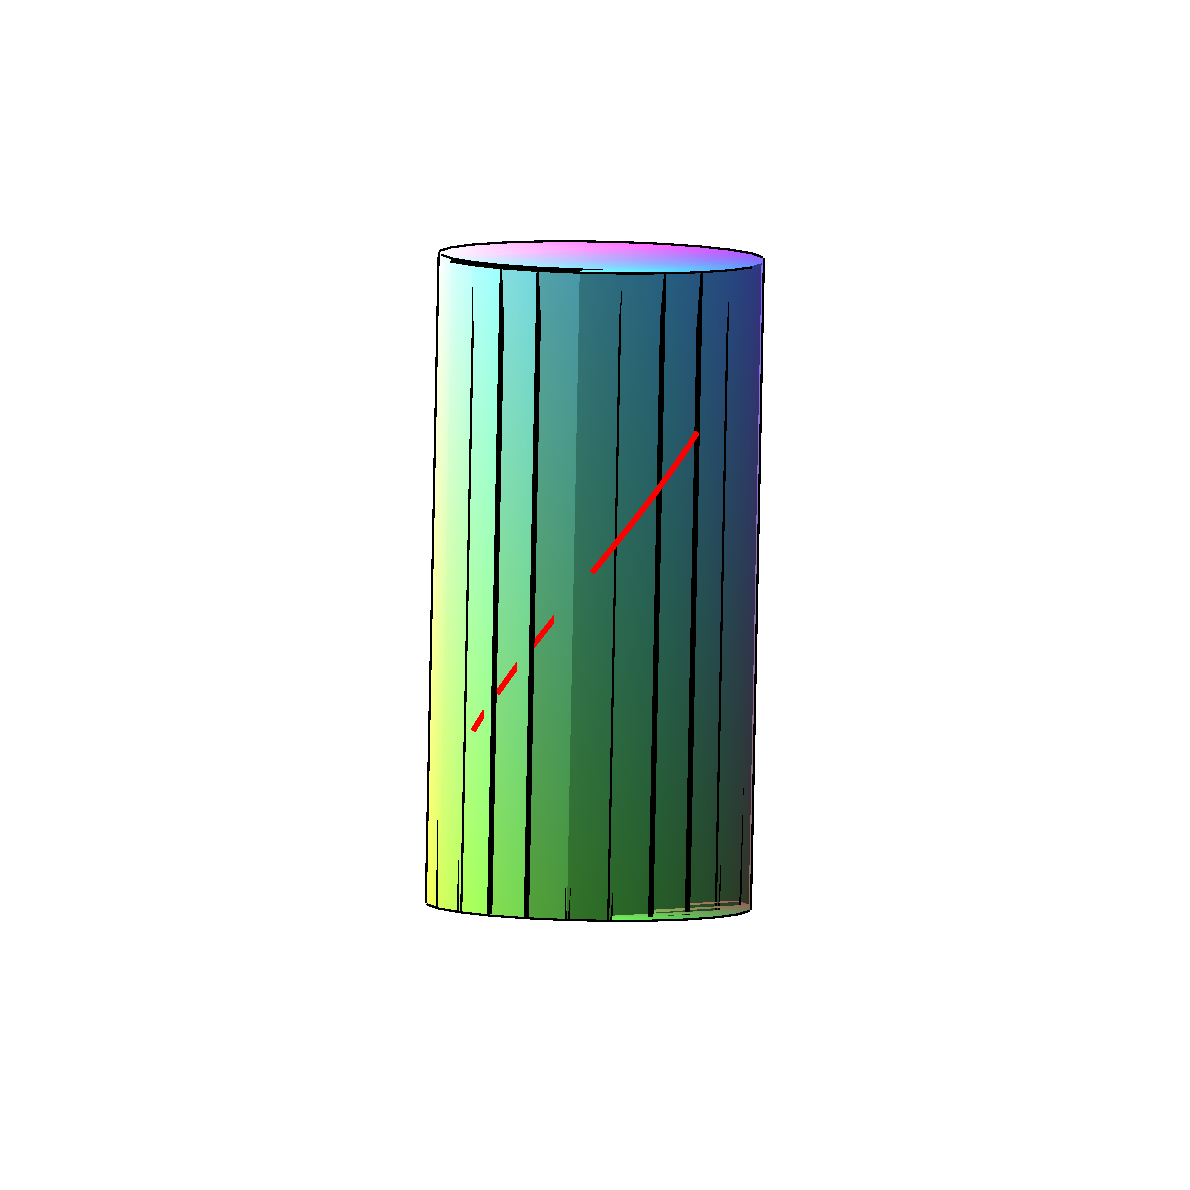
\includegraphics[scale=0.4]{pictures/Opg8_Fig1.eps}
\caption{lol hurr durr+}
\end{figure}
Som det er beregnet og kan ses, ligner det ganske rigtig den korteste vej over cylinderfladen mellem de 2 punkter og derved en geodætisk kurve.
\\
\\
\\
Vi kan nu se hvad det betyde at $Z_a=Z_b$, $Z_a$ til 5 og vi sætter $\theta_a$ til $\frac{1}{2}\pi$ $\theta_b$ til $\pi$ og hertil foretager de samme beregniner som eksemplet tidligere.
\begin{lstlisting}
> with(plots);
> Curve1 := spacecurve([cos(t), sin(t), 4*t/Pi+1], t = theta[a] .. theta[b], color = red);

> with(plottools);
> display(cylinder([0, 0, 2], 1, 4), Curve1, orientation = [45, 70], scaling = constrained);
\end{lstlisting}
\begin{figure}[h!]
\center
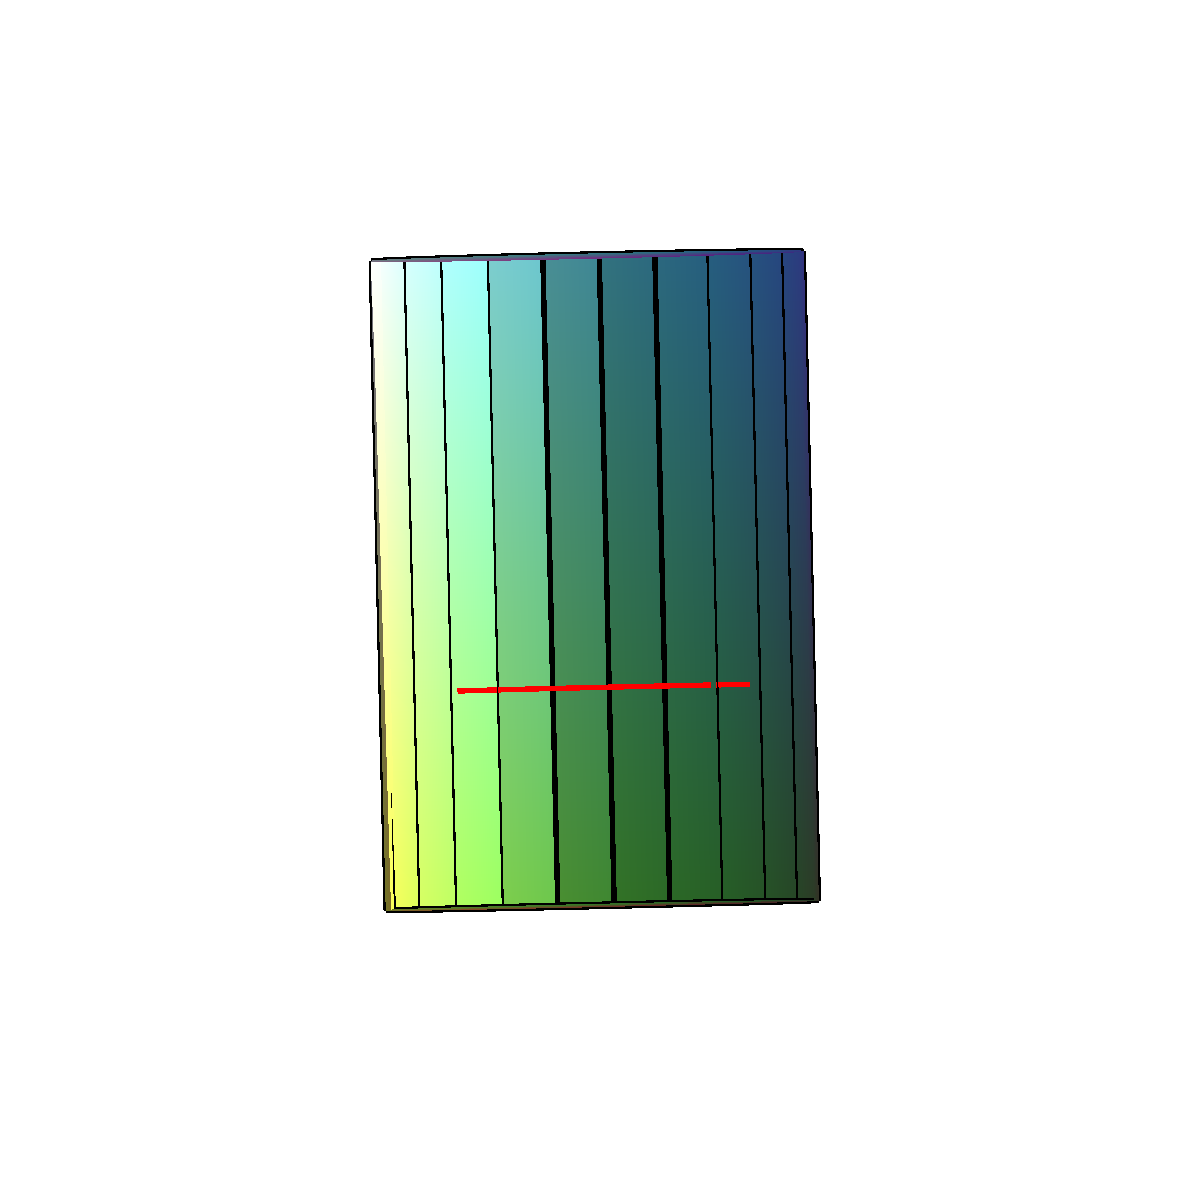
\includegraphics[scale=0.4]{pictures/Opg8_Fig2.eps}
\caption{lol hurr durr+}
\end{figure}
Som det ses bliver det en vandret strej mellem de 2 punkter, som er resultatet af at $\delta Z$ bliver 0.
\\
\\
\\
Vi skal nu se hvad der sker hvis vi ændrer $\theta$. Hertil sætter vi $\theta_a$ til $\frac{4}{3} \pi$ og $\theta_b$ til $\frac{4}{3}$ og vi sætter $Z_a$ til 3 og $Z_b$ til 5
\begin{lstlisting}
> with(plots);
> Curve1 := spacecurve([cos(t), sin(t), 3*t/(2*Pi)+2], t = 0 .. (4/3)*Pi, color = red);

> with(plottools);
> display(Curve1, orientation = [45, 70], scaling = constrained);
\end{lstlisting}
\begin{figure}
\center
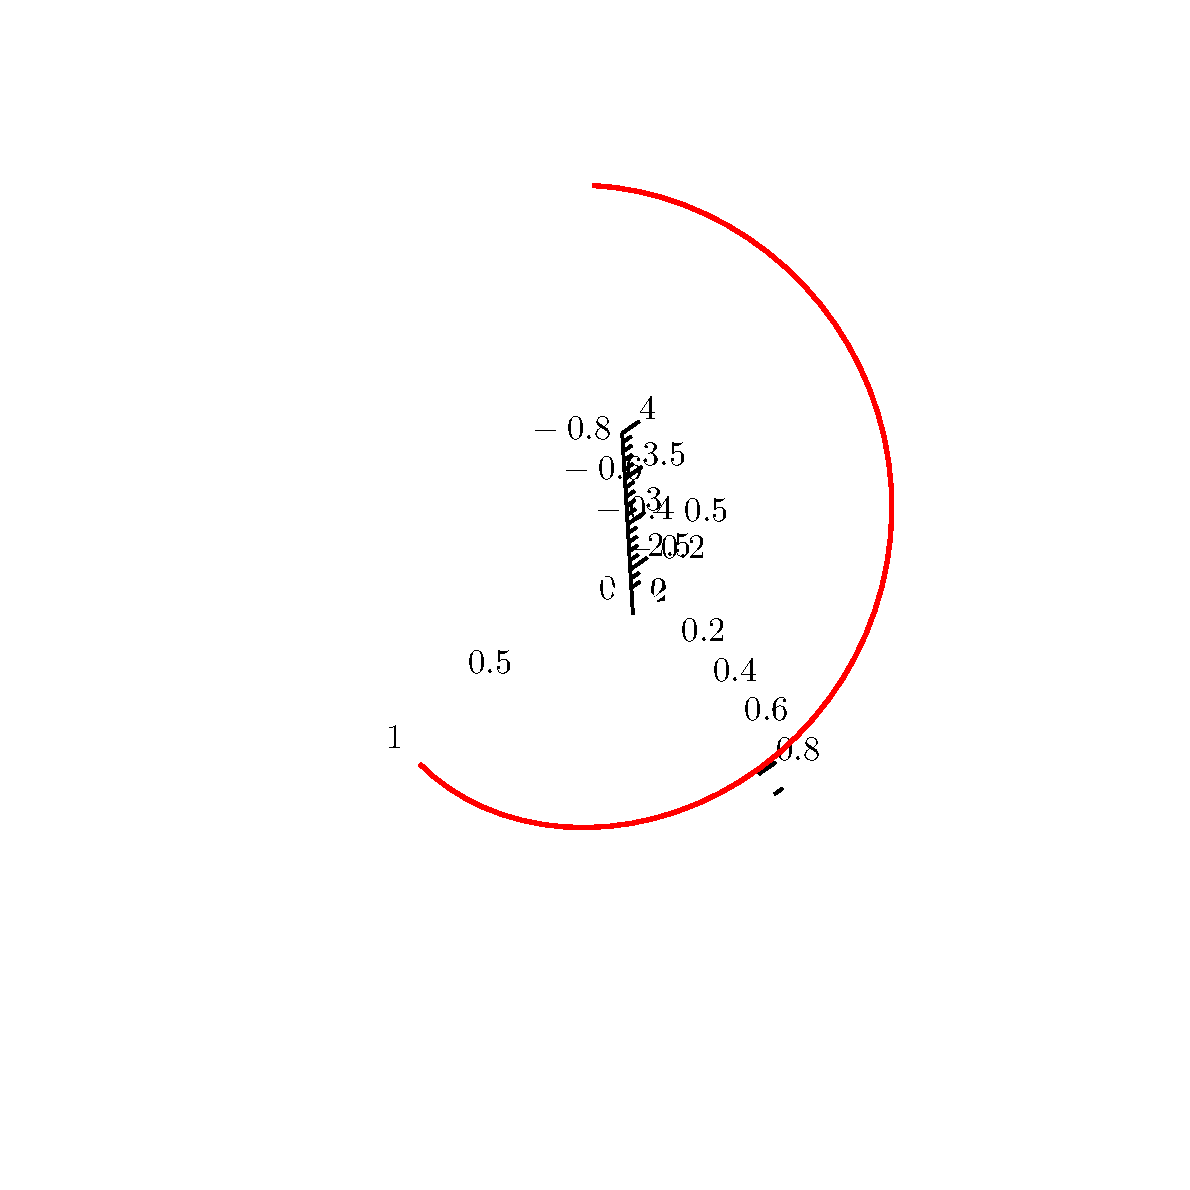
\includegraphics[scale=0.4]{pictures/Opg8_Fig3.eps}
\caption{lol hurr durr+}
\end{figure}
Af forståelsesmæssige grunde er cylinderen blivet fjernet og er samtidig fremhæve pointen.
\\
I dette tilfælde er der beregnet hvad der eftersigende skulle være den korteste vej fra punkt A til B, men dette tilfældet havde $\theta_a$<$\theta_b$ ikke været gældende. Var der ikke givet nogle restriktioner skulle den geodætiske kurve gået venstre rundt om z aksen.
\\
Et interessant tilfælde forekommer når 2 punkter befinder sig lige over hinanden, dette vil nemlig resultere i at hældningen mellem de 2 punkter bliver uendelig.
\\
\\
\\
Vi kan nu se hvad det betyder at $\theta_a=\theta_b$. Vi sætter $\theta_a-b$ til $\pi$, $Z_a$ til 3 og $Z_b$ til 3 og $Z_b$ til 5 og hertil foretager de samme beregniner som eksemplet tidligere.
\\
Udtryk for hældningen
\begin{equation}
k=\frac{3-5}{\pi-\pi}
\end{equation}
Dette ligning vil resultere at hældning bliver uendelig
\begin{lstlisting}
> with(plots);

> Curve1 := spacecurve([cos(t), sin(t), k*t+C], t = theta[a] .. theta[b], color = red);
> with(plottools);
> display(cylinder([0, 0, C], 1, 5), Curve1, orientation = [45, 70], scaling = constrained);
\end{lstlisting}
\begin{figure}
\center
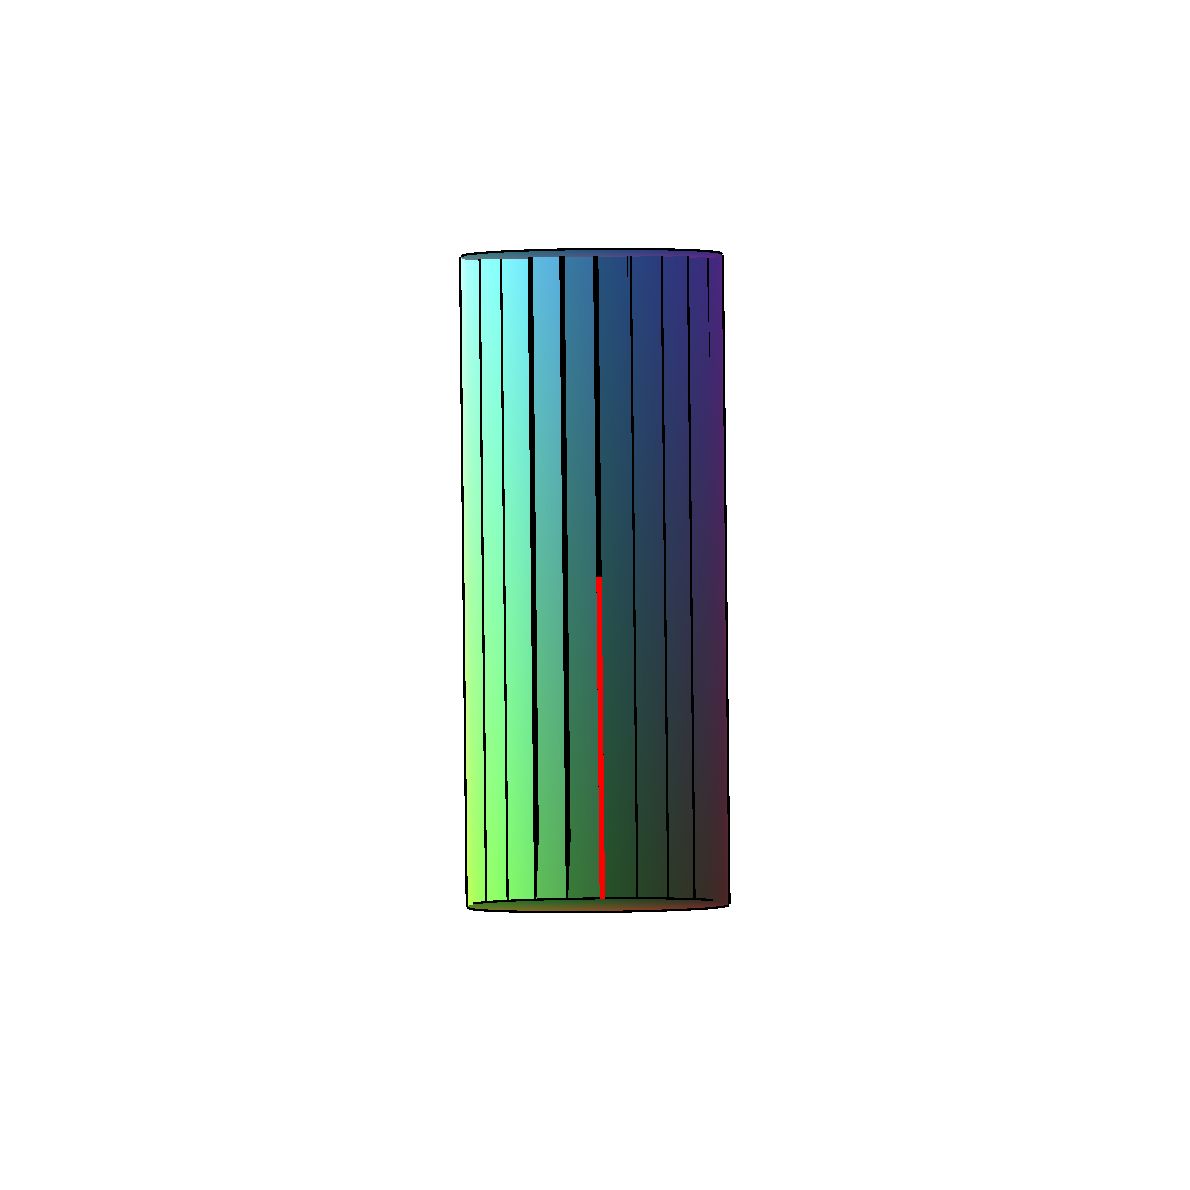
\includegraphics[scale=0.4]{pictures/Opg8_Fig4.eps}
\caption{lol hurr durr+}
\end{figure}
Som det fremgår forbindes de 2 punkter nu af en ret linje.

